\documentclass[a4paper,oneside]{article}
\usepackage{indentfirst}
\usepackage[top=0.7in, bottom=0.7in, left = 0.7in, right = 0.7in]{geometry}
\usepackage{graphicx}
\usepackage{subcaption}
\usepackage{indentfirst}
\usepackage{cite}
\usepackage{fontspec}

\title{Term Project\\Splitter: Mining Fine-Grained Sequential Patterns in Semantic Trajectories}
\author{Fawwaz Dzaky Zakiyal (201899213)\\Tanjung Dion (201883621)\\}
\date{Stream Database (Fall 2018)}

\begin{document}
	\maketitle
	
	\section{Introduction}
	Semantic trajectory is a sequence of timestamped places wherein each place has information about spatial location and a semantic label. By mining fine-grained pattern that satisfy semantic consistency (consistent place id in each category), spatial compactness (compact area for each category) and temporal continuity (limited time constraint), it will give benefit such as urban planning and targeted advertising. This process of mining fine-grained pattern have been proposed by Zang et. al \cite{splitter}. For the final project we will re-implement the process of find fine-grained pattern in Java programing language.
	
	\section{Problem}
	\begin{itemize}
		\item How to mine the coarse patterns and their snippets? 
		\item How to effectively cluster the snippets given the fact that we do not know the correct number of clusters?
	\end{itemize}
	
	 
	\section{Proposed Method}
		 \subsection{Dataset}
		 This project will use the real dataset, 4SQ that collected from Foursquare check-in sequence in New York. It consists of 48564 places that divided into 417 place categories and it stored semantic trajectories from 14909 users. 4SQ dataset provides 3 files:
		 \begin{enumerate}
		 \item \textit{Sequences}, it contains users semantic trajectories including attributes of check-in timestamp and place ID.
		 \item \textit{Places}, it contains information about the places (place ID, latitude, longitude, category ID).
		 \item \textit{Category}, it contains information of place category ID corresponding with its place category name.
		 \end{enumerate}

		 \subsection{System Design}
		 	\begin{figure}[!ht]
		 	\centering
		 	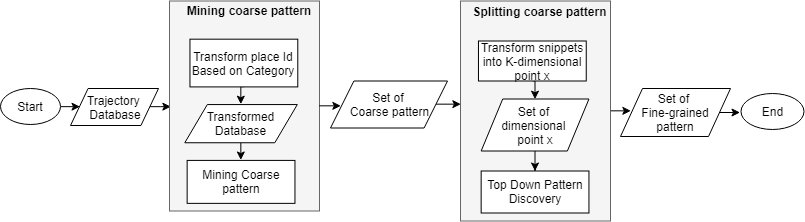
\includegraphics[width=1\linewidth]{splitter}
		 	\caption{System Design}
		 	\label{fig:systemdesign}
		 \end{figure}
		 Figure \ref{fig:systemdesign} show the process of mining fine-grained pattern in semantic trajectories. This method consist of two part: mining coarse pattern and splitting coarse pattern. Mining coarse pattern is a process to find sequential pattern that satisfy semantic consistency and temporal continuity. In the first step, we add trajectory dataset that have information about place id, movement time, group id, and spatial location to the system. This trajectory dataset will be transformed into semantic trajectory dataset by grouping place id based on category. However, we still keep the original place id in each category to prevent one trajectory from being counted repeatedly. By doing this process, our trajectory dataset will satisfy semantic consistency.
		 
		 Then, Prefixspan algorithm will be used to mining the coarse pattern. In the Prefixspan algorithm, we include all posfixes to avoid missing pattern under the given time constrain. Output from mining coarse pattern is set of coarse pattern that will be used in the next process. The next process is finding fine-grained pattern that satisfy spatial compactness in by splitting a coarse pattern in top down manner. Set of coarse pattern from previous process will be transformed into K-dimensional point x.
		 
		 Then, we employ mean shift clustering to extract the dense and compact snippet cluster based on the support and variance threshold. To speed up the process, the unqualified snippet cluster will be organized into several disjoint communities. By only clustering each communities, we can gradually reduce the kernel windows in clustering method to speed up the clustering process.
		
		\subsection{Implementation}
		We will re-implement the process of mining fine-grained pattern using java programing language. The user interface of program will be provided as shown in the Figure \ref{fig:UI}. Figure \ref{fig:javagui} shows the illustration of our program. There are an dataset input in csv format, 4 parameters input,  show button for showing graph representation like in the figure \ref{fig:graph}, and 3 button to start the process individually or start all of the process respectively. 
		
		\begin{figure}[!h]
			\centering
			\begin{subfigure}[b]{0.4\linewidth}
				\centering
				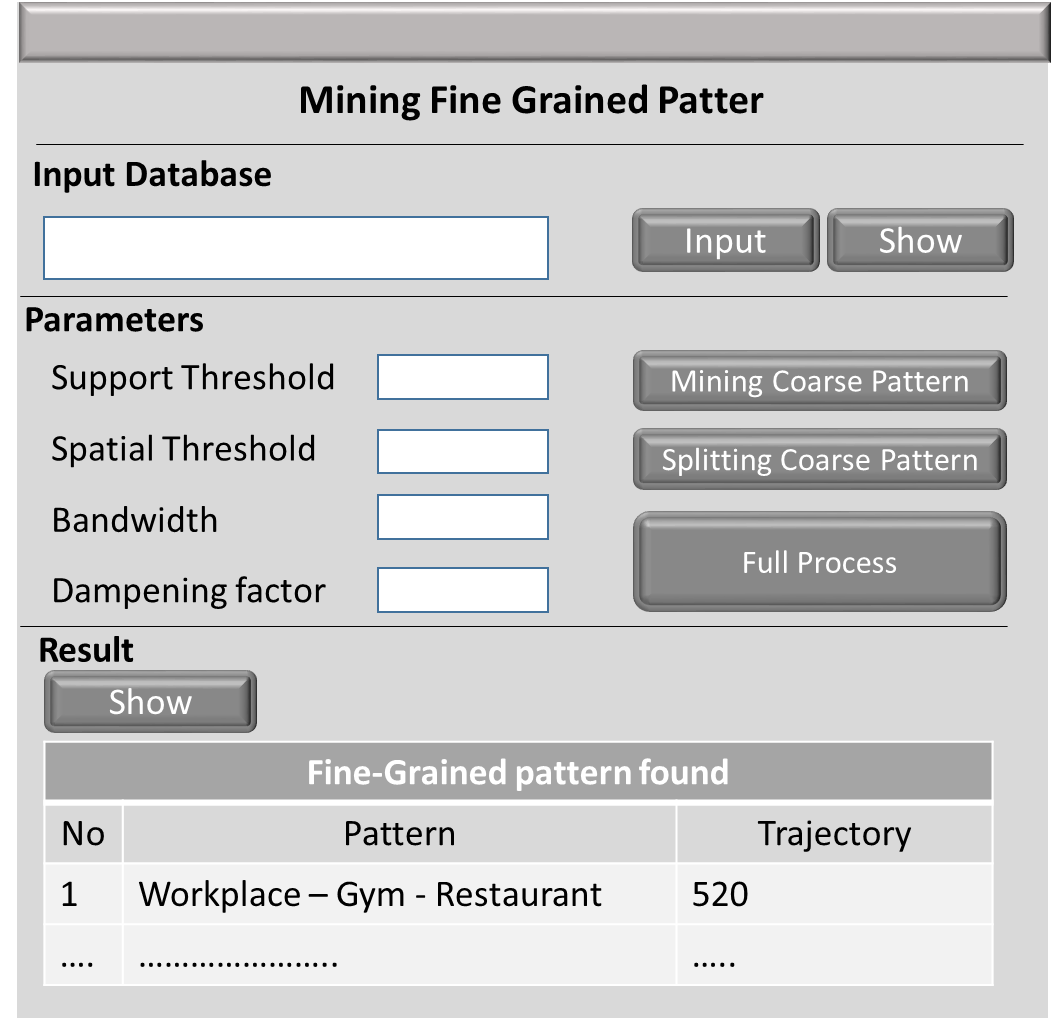
\includegraphics[width=1\linewidth]{GUI}
				\caption{Program UI illustration}
				\label{fig:javagui}
			\end{subfigure}
				\begin{subfigure}[b]{0.4\linewidth}
				\centering
				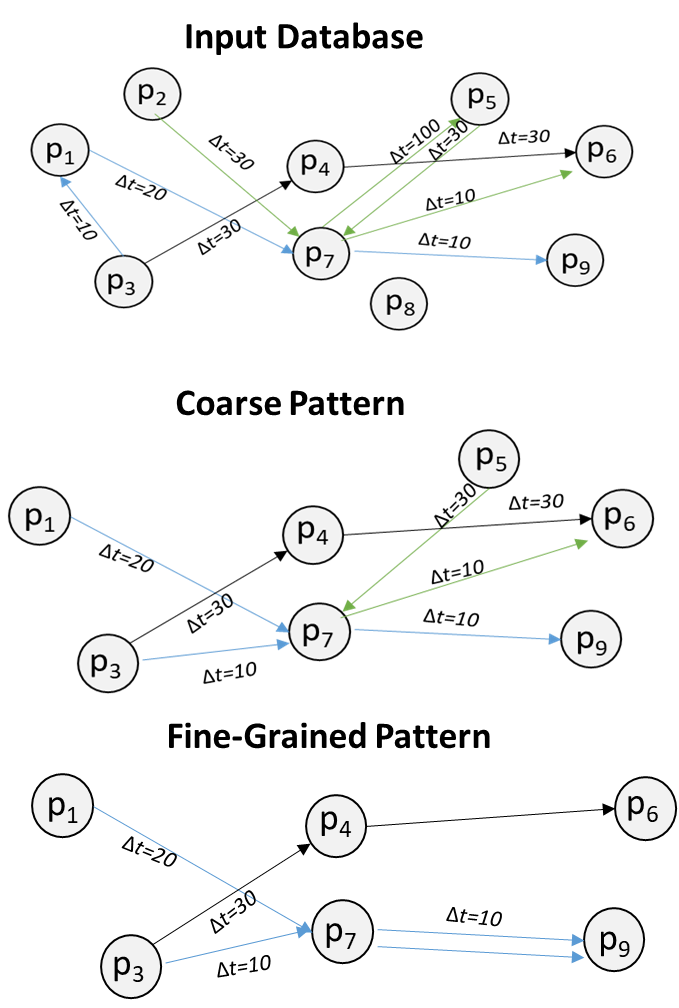
\includegraphics[width=0.7\linewidth]{GraphRepresentation}
				\caption{Graph illustration}
				\label{fig:graph}
			\end{subfigure}
			\caption{User Interface Ilustration}
			\label{fig:UI}
		\end{figure}
		
		
	\section{Testing and Evaluation}
	For the testing and evaluation, we will conduct an experiment of mining fine-grained pattern by varying support threshold, spatial variance threshold, time movement constraint, kernel windows size, and dampening factor in the term of coverage and pattern. Coverage is the total number of trajectory in all pattern that satisfy fine-grained pattern. 
\begin{thebibliography}{1}
	\bibitem{splitter} Zhang, C., Han, J., Shou, L., Lu, J., La Porta, T. (2014).{\em Splitter: Mining fine-grained sequential patterns in semantic trajectories}. Proceedings of the VLDB Endowment, 7(9), 769-780.
\end{thebibliography}
\end{document}